\section{Un coup de marteau (3 points)}\label{marteau}

Jeanne pose du plancher. Elle cherche à comprendre ce que subit le clou lorsqu'on vient le frapper avec le marteau.

\begin{questions}
	\question \'Etablir un diagramme objet-interaction pour l'objet <<clou>>.
		\begin{solution}
			\begin{center}
				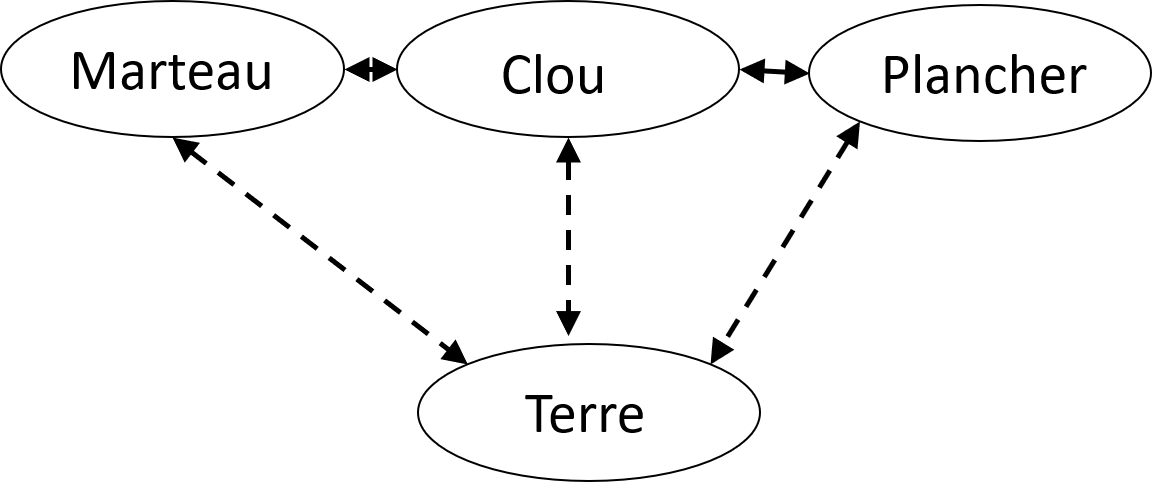
\includegraphics[scale=0.5]{doi_marteau}
			\end{center}
		\end{solution}
	\question Faire un schéma de la situation et représenter les forces qui s'exercent sur le clou.
	\question Quel est l'effet de l'ensemble des actions qui s'exercent sur le clou.
		\begin{solution}
			L'ensemble des actions qui s'exercent sur le clou fait qu'il s'enfonce dans le plancher.
		\end{solution}
	
\end{questions}

\subsection*{Données}
	\begin{itemize}
		\item Force exercée par le marteau sur le clou : \num{50000} N;
		\item Force exercée par la planche sur le clou : \num{5000} N;
		\item \'Echelle : 1 cm $\leftrightarrow$ \num{10000} N.
	\end{itemize}